\documentclass{article}

\usepackage[utf8]{inputenc}
\usepackage{amsmath} 
\usepackage{amsfonts}
\usepackage{graphicx}
\usepackage{tabularx}
\usepackage{array}
\usepackage{booktabs}


\graphicspath{ {./output/} }

\author{Paulo Gugelmo Cavalheiro Dias}
\title{Master Thesis: Climate change economic effect on health through temperature}

\begin{document}

\maketitle

\tableofcontents

\section{Introduction}

\subsection{Introduction to the subject}

Climate change is projected to strongly impact temperature distribution in the upcoming century. 
Therefore, it is important to try to identify the different effects of temperature on the economy.
One of the particular effect channels is health. 
How will temperature change affect the health status of the population, and therefore the economic production?

\subsection{Related literature}

In order to study this question, 

The relationship between temperature, health, and economics is deeply intricated 
in several literature fields. 

First, since the 2000s, the relationship on how climate and economics are intertwined has been studied in a more climate-related literature.

Second, health economics has identified important findings in the last years.

- Health economics: 
    - Health and productivity.
    - Health and life expectancy.
- Climate and economics: 
    - Hotter temperature and conflicts. 


\subsection{Research question and strategy}

The goal of this Master Thesis is to propose a simple approach to model the effect
of temperature on the health of individuals, and subsequently on the economy. 

In order to achieve this, two main parts are identified. 

First, an empirical part studying the link between temperature and health will be done. 

Second, a macroeconomic model is presented to explain the economic mechanisms that will be affected by the identified empirical relationships.

\section{Setting}

This section is dedicated to the presentation of the general setting
in which individuals live in this model.
First, the relationships between the different elements in a general framework will be presented.
Then, the data used will be presented and discussed. 
The methods used to estimate the functional forms of the relationships will then be 
presented, and will be refered as the specific case of this work.
Finally, results of the estimation process of these relationships will be presented and discussed.

\subsection{Goal}

\subsection{Formal Description}

At each period, an exogenous weather realization occurs, and individuals draw a health and living status. 

\subsubsection{History vectors}

In a general framework, we can think of the health of an individual at time $t$ as a vector $\mathcal{H}_t\in \mathbb{R}^{t}$ containing
all the health status of the individual throughout their life.
Similarily, we can think of the weather experienced by an individual at time $t$ as a vector $\mathcal{W}_t\in \mathbb{R}^{t}$ containing
all the weather conditions experienced by the same individual throughout their life.

\subsubsection{Health Status}

Let $H_{t}\in\Omega(H)$ be a random variable denoting the health status of an individual at time $t$.
The functional form of its distribution $f_{h}$ will depend on its sample space $\Omega(H)$. 
The past health history and the temperature also affect the probability distribution of health status.
Generically, we can therefore write: 

\begin{equation}
    H_{t}\sim f_{h}(\mathcal{H}_{t-1},\mathcal{W}_t)
\end{equation}


\subsubsection{Living Status}

Let $L_{t}\in\{0,1\}$ be a random binary variable denoting the living status of an individual at time $t$.
It is determined by a Bernoulli distribution with parameter $p_t$ such that: 

\begin{equation}
    L_{t} \sim \mathcal{B}(p_{t})
\end{equation}

The probability parameter $p_{t}$ depends on their health, age, and temperature.
In a general approach, we can rewrite the first equation such as: 

\begin{equation}
    L_{t} \sim \mathcal{B}(p_{t}(\mathcal{H}_t,\mathcal{W}_t))
\end{equation}

As such, the probability of an individual to be alive at period $t$ is: 

\begin{equation}
    Pr(L_t = 1 | \mathcal{H}_t,\mathcal{W}_t ) = \prod_{j = 1}^{t} p_{j}(\mathcal{H}_j,\mathcal{W}_j)
\end{equation}

\subsection{Data}

Three main datasets were used to estimate the mentioned relationships: 
the Health and Retirement Study (HRS) dataset for
health status and survival,
the Berkeley Earth dataset,
and finally the Federal Reserve Bank of Saint Louis (FRED) dataset for 
other economic variables.

\subsubsection{HRS Data}

The HRS data 

\begin{tabular}{ccccc}
    \toprule
    variable & mean & min & median & max\\
    \midrule
    Year & 2010.28 & 2002.00 & 2010.00 & 2018.00\\
    Age & 68.11 & 11.00 & 67.00 & 112.00\\
    Health & 2.95 & 1.00 & 3.00 & 5.00\\
    Status & 0.96 & 0.00 & 1.00 & 1.00\\
    GDP & 15759.15 & 10929.11 & 15048.97 & 20656.52\\
    Temperature & 0.55 & 0.40 & 0.52 & 0.73\\
    \bottomrule
\end{tabular}
    

\subsubsection{Climate Data}

\begin{figure}[h]
    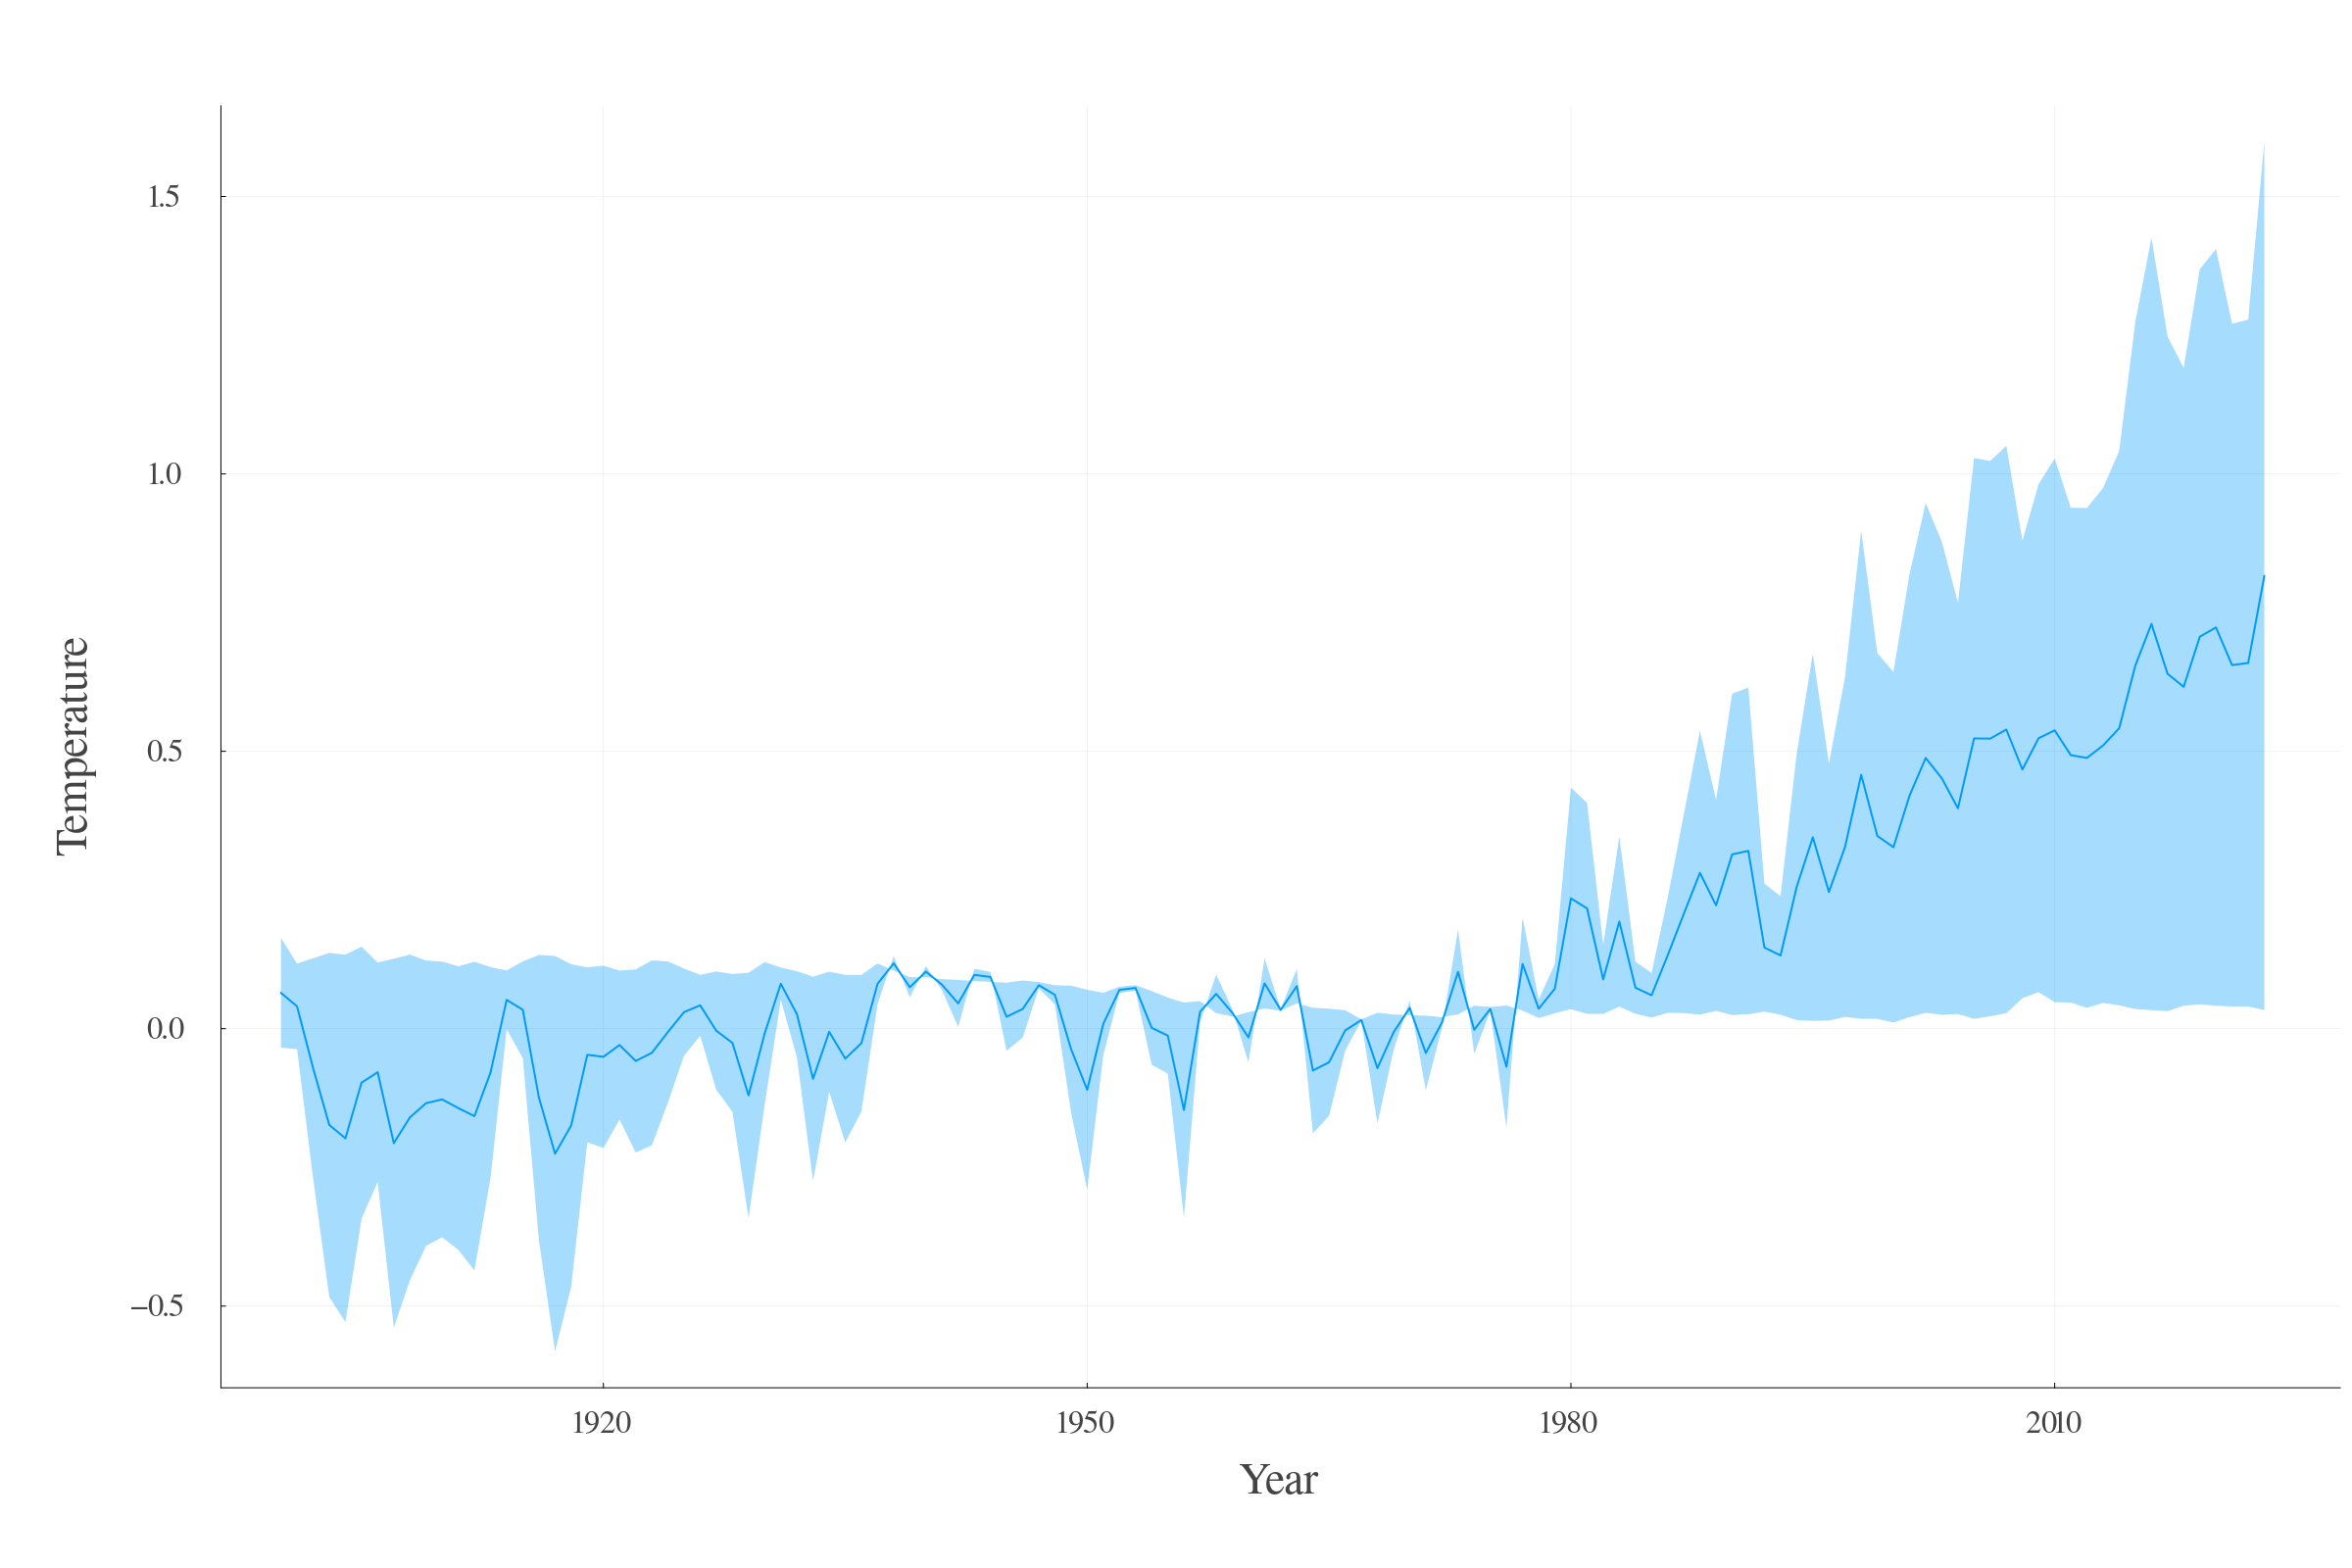
\includegraphics[width=\textwidth]{/Users/paulogcd/Documents/Master_Thesis/working_elements/Draft/output/figure_1.png}
    \caption{Average annual temperature from the Berkeley Dataset}
    
    The light blue area is delimited by the anomalies extrema of each year, and
    the dark blue line represents the average of the anomalies.
\end{figure}

\subsection{Methods}

\subsubsection{Health Transition}

The HRS dataset provides rich information regarding the health status of individuals. 
To make use of the five different values of the self reported health, it was therefore decided not to
recode the variables into a binary health status variable $H\in\{Bad, Good\}$. 

\subsubsection{Living Status}

The living status variable, being binary, did not represent a challenge
as great as the health transition estimation. 

A simple logistic regression on age and health status yields findings similar with the
rest of the literature. 

\begin{figure}[ht]
    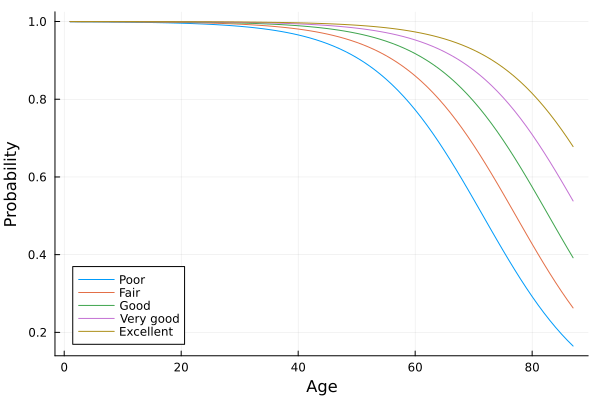
\includegraphics[width=\textwidth]{/Users/paulogcd/Documents/Master_Thesis/working_elements/Draft/output/figure_2.png}
    \caption{Annual probability of survival as a function of age and health status}
\end{figure}


\subsection{Estimates}

\section{Model}

\subsection{Baseline specification }

The agents maximizes: 

$$ \max_{c_{t},l_{t},s_{t+1}}{\mathbb{E}\left[\sum_{t=1}^{100} \beta^{t}\cdot u(c_t,l_t)\right]}$$

Their utility function is: 

$$u(c_{t},l_{t}) = \frac{c_{t}^{1-\rho}}{1-\rho}-\xi_{t}\cdot \frac{l_{t}^{1+\varphi}}{1+\varphi}$$

With : 

-  $c$  the consumption

-  $l$  the quantity of labor supply provided by the agent

-  $h$  the health status

-  $w$  the weather variable, which is here temperature

-  $\xi$ the labor disutility coefficient

The agent is subject to: 

$$c_{t} + s_{t+1} \leq l_{t}\cdot z_{t} + s_{t}\cdot(1+r_{t})$$

With: 

-  $c_t$ the consumption at period $t$

-  $s_{t+1}$ the savings for period $t+1$

-  $l_t$ the labor supply provided by the agent at period $t$

-  $z_t$ the productivity at time $t$

-  $s_{t}$ the savings available at the beginning of period $t$

-  $r_{t}$ the interest rate at period $t$

Also, let us define the borrowing constraint as: 

$$s_{t+1}\geq \underline{s}, \forall t$$

\subsection{Numerical methods}

\section{Results}

\section{Conclusion}

\section{References}

\section{Appendix}

\end{document}